\section{Arquitectura TP1}
A continuación detallamos la arquitectura diseñada en base al enunciado del TP1.

\subsection{Paneo General}
\begin{center}
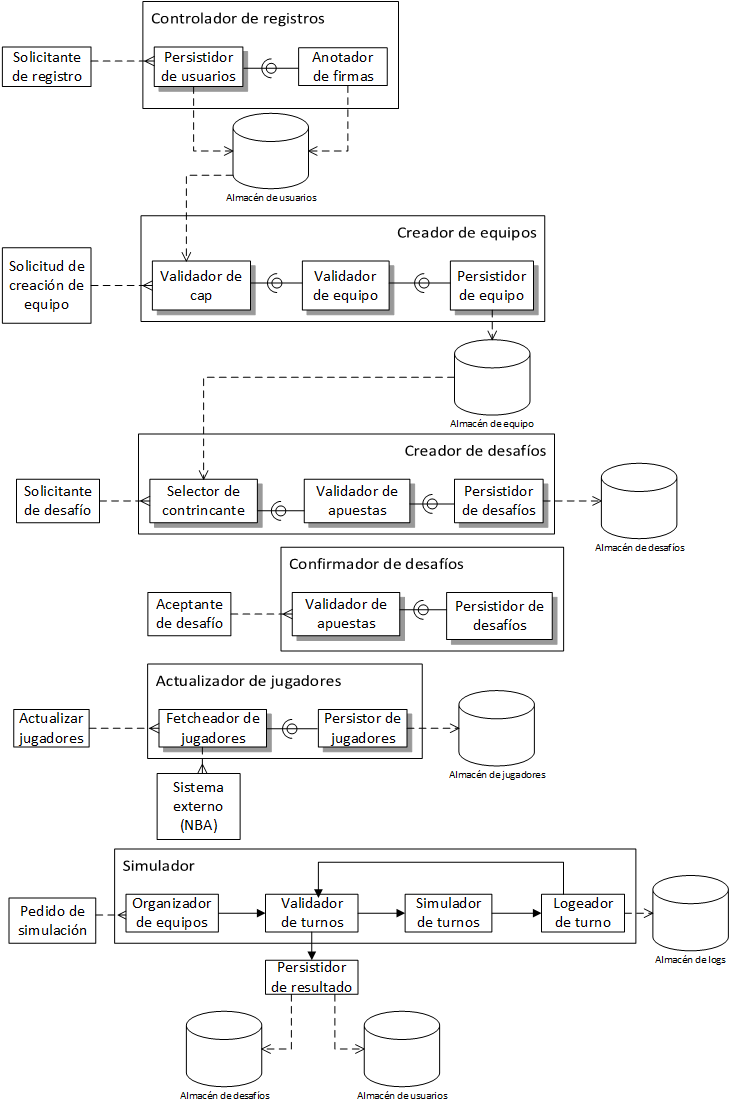
\includegraphics[scale=0.70]{diagramas/tp1/arquitectura_tp1.png}
\end{center}
\label{fig:arquitectura_tp1}

En la figura \ref{fig:arquitectura_tp1} se ven los principales componentes del sistema, sobre los cuales se hace zoom en las secciones posteriores, además de los repositorios utilizados para nuestra solución.

\subsection{Actualizador de jugadores}
\begin{center}
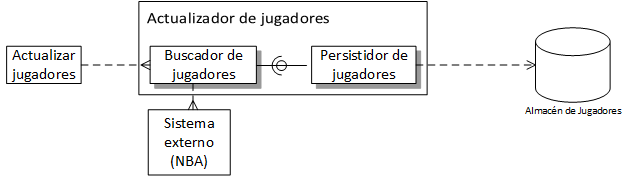
\includegraphics[scale=0.80]{diagramas/tp1/buscadordejugadores.png}
\end{center}
\label{fig:buscadordejugadores}

Dado que existe la posibilidad de actualizar las estadísticas de los jugadores mediante un sistema externo, un administrador podrá realizar esta solicitud que será enviada directamente al \emph{Buscador de jugadores}, que se conectará directamente con el sistema externo para traer la última versión de los datos correspondientes. Esta será enviada directamente al \emph{Persistidor de jugadores}, que se encargará de actualizar la información de los mismos o agregar nuevos, según sea necesario.

\subsection{Creador y confirmador de desafios}
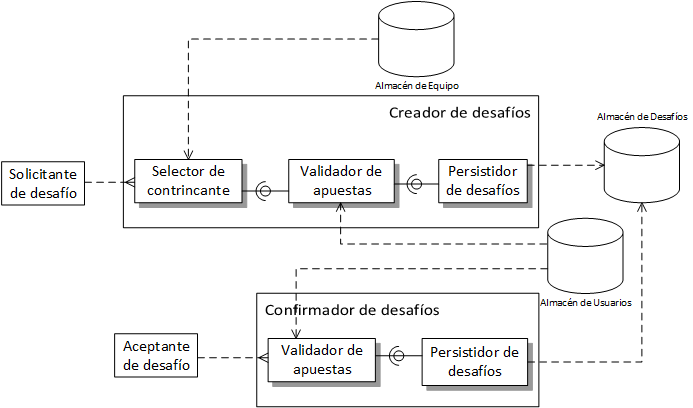
\includegraphics[scale=0.80]{diagramas/tp1/desafios.png}
\label{fig:desafios}

Cuando un usuario solicite desafiar a otro, se enviará la información correspondiente a un componente \emph{Selector de contrincantes} que se encargará de buscar toda la información correspondiente a ambos equipos y la enviará al \emph{Validador de apuestas}. Este último será quien deba confirmar que ambos participantes cuentan con las fichas necesarias (por lo menos en primera instancia), para poder participar del desafío y descontará las fichas necesarias del usuario que solicitó el desafío.

Cuando el participante desafiado acepte alguno de los desafíos que se le envían, la comunicación se enviará directamente hacia el \emph{Validador de apuestas}. Este componente validará una vez más que el equipo desafiado cuente con las fichas necesarias (para que no se dé el caso en que, luego de haber sido desafiado, haya gastado sus fichas en otros desafíos) y luego se comunicará con el \emph{Persistidor de desafíos} para que el desafío sea finalmente confirmado, ya por ambas partes.

\subsection{Creador de equipos}
\begin{center}
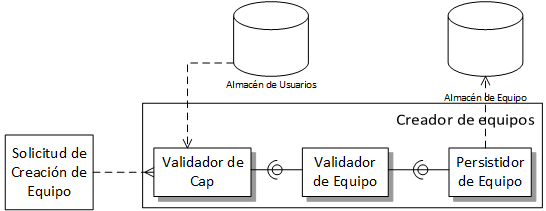
\includegraphics[scale=0.80]{diagramas/tp1/equipo.png}
\end{center}
\label{fig:equipo}

Toda comunicación que se realice con el fin de crear un nuevo equipo, dará inicio a través de un componente \emph{Validador de CAP} que se encargará, mediante la verificacion de los datos almacenados en el repositorio de usuarios, de confirmar que el usuario cuenta con el CAP necesario para poder formar dicho equipo. Un segundo componente (\emph{Validador de equipo}), recibirá la confirmación de este y tendrá como función la de validar la información concreta del equipo (están todas las posiciones ocupadas, jugador estrella elegido, etc.) para luego enviarla al \emph{Persistidor de equipos} que se encargará de almacenarla en el repositorio correspondiente (\emph{Almacén de equipos}).

\subsection{Controlador de registros}
\begin{center}
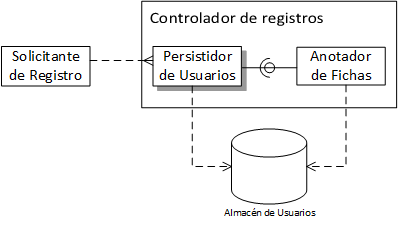
\includegraphics[scale=0.80]{diagramas/tp1/registros.png}
\end{center}
\label{fig:registros}

Toda solicitud de registro de un nuevo usuario es recibida por el \emph{Persistidor de usuarios}, encargado de almacenar los datos del mismo en el repositorio \emph{Almacén de usuarios} y de enviar un mensaje hacia el \emph{Anotador de fichas} que persiste la cantidad de fichas otorgadas al nuevo usuario. El objetivo de mantener estos dos componentes separados es el de ofrecer flexibilidad en el manejo de las fichas y ofrecer la posibilidad de cambiar este módulo con bajo impacto en el sistema.

\subsection{Simulador}
\begin{center}
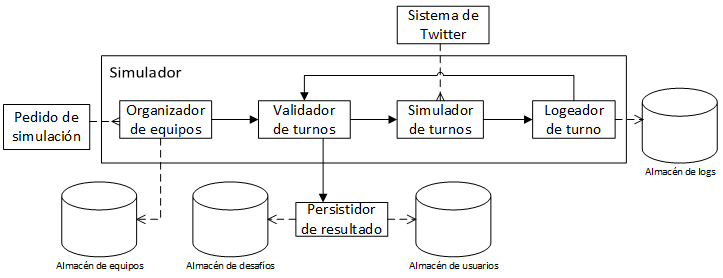
\includegraphics[scale=0.80]{diagramas/tp1/simulador.png}
\end{center}
\label{fig:simulador}

Cuando un nuevo pedido de simulación llegue al sistema, será recibido por un \emph{Organizador de equipos}. Este componente traerá la información de los dos equipos comprometidos en el desafío y se la enviará al \emph{Validador de turnos}. Este componente, que es parte de un ciclo de ejecución, validará que la cantidad de turnos total configurada en el sistema todavía no se haya cumplido y en caso de que todavía haya pendientes, notificará al \emph{Simulador de turnos}. A través de una comunicación directa con el API de Twitter, este componente calculará los resultados de las simulaciones del turno correspondiente. Estas se irán enviando una tras otra hacia el \emph{Logeador  de turnos} que persistirá los datos para que luego estén disponibles para los usuarios. Cuando este componente termine de cumplir su función, notifica una vez más al \emph{Validador de turnos}, para que este revise si todavía quedan pasos por simular. En caso de que esto no sea así, se comunicará con el \emph{Persistidor de resultados}, encargado de almacenar el resultado del desafío y la nueva posición (o el cambio de puntos) de los usuarios participantes.
